\documentclass{article}
\usepackage[utf8]{inputenc}
\usepackage{graphicx}
\graphicspath{ {./images/} }

\title{Labwork 01}
\author{Group 10}
\date{February 2021}

\begin{document}
\maketitle
\section{Design Protocol}
\begin{figure}[ht]
\centering
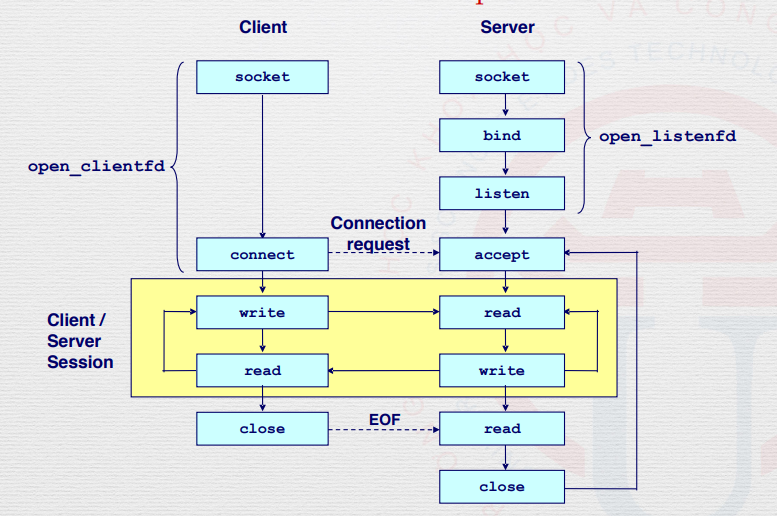
\includegraphics[scale=0.35]{protocol.PNG}
\caption{Protocol}
\end{figure}

\section{System organization}
Server:
\begin{itemize}
\item create socket
\item bind to port
\item listen to client
\item Accept connect request from client
\item Load file content from server and send to client
\item Receive file from client
    
\end{itemize}
Client:
\begin{itemize}
\item create socket
\item connect to server port
\item load file content from computer and send to server
\item read and write file content sent from client.
\end{itemize}
\section{Implementation}
We do 2 code file client.c and server.c depend on socket chat system - server and socket chat system - client 

\end{document}
